\documentclass[]{article}
\usepackage[round]{natbib}

\usepackage[margin=1in]{geometry}
\usepackage{url} 
\usepackage{authblk}
\usepackage{graphicx}
\usepackage{color}
\usepackage{booktabs}
\usepackage{xspace}

\usepackage{amsmath,amssymb}
\usepackage{longtable,booktabs,array}


\newcommand{\E}{\mathbb{E}}
\newcommand{\moments}{\texttt{moments}\xspace}
\newcommand{\Relate}{\texttt{Relate}\xspace}
\newcommand{\msprime}{\texttt{msprime}\xspace}

\newcommand{\comment}[1]{{\textcolor{red}{APR: #1}}}

% cross-reference with supplement
\usepackage{xr}
\externaldocument{supplement}

\begin{document}

\title{A heterogeneous landscape of selection and epistasis in protein-coding genes revealed by two-locus statistics}
\author[]{Aaron P. Ragsdale}
\affil[]{Department of Integrative Biology, University of Wisconsin, Madison, WI, USA}
\affil[]{apragsdale@wisc.edu}
\maketitle


\begin{abstract}

Selected mutations interfere and interact with evolutionary processes at nearby
loci, distorting allele frequency trajectories and creating correlations
between pairs of mutations. A number of recent studies have used patterns of
linkage disequilibrium (LD) between selected variants to test for selective
interference and epistatic interactions, with some disagreement over
interpreting observations from data. Interpretation is hindered by a lack of
analytic or even numerical expectations for patterns of variation between pairs
of loci under the combined effects of selection, dominance, epistasis, and
demography. Here, I develop a numerical approach to compute the expected
two-locus sampling distribution under diploid selection with arbitrary
epistasis and dominance, recombination, and variable population size. I use
this to explore how epistasis and dominance affect expected signed LD,
including for non-steady-state demography relevant to human populations. Using
whole-genome sequencing data from humans, I explore genome-wide patterns of LD
within protein-coding genes. I show that positive LD between missense mutations
within genes is driven by strong positive allele-frequency correlations between
pairs of mutations that fall within the same annotated conserved domain,
pointing to compensatory mutations or antagonistic epistasis as the prevailing
mode of interaction within conserved genic elements. LD between missense
mutations is reduced outside of conserved domains, as would expected under
Hill-Robertson interference. The heterogeneous landscape of both mutational
fitness effects and selective interactions within protein-coding genes calls
for more refined inferences of the joint distribution of fitness and
interactive effects, and the methods presented here should prove useful in that
pursuit.

\end{abstract}

\section{Introduction}\label{sec:introduction}

Most new mutations that affect fitness are deleterious and tend to be
eliminated from a population. The amount of time that a deleterious mutation
segregates depends on the strength of selection against genomes that carry it,
with very damaging mutations kept at low frequencies and purged relatively
rapidly. In the time between mutation and fixation or loss, selected variants,
both beneficial and damaging, can dramatically impact patterns of variation in
nearby linked regions \citep[e.g.][]{Smith1974-em,Charlesworth1995-dq,Kim2000-on}.
This distortion away from neutral expectations has been empirically documented
using sequencing data from an ever-growing set of study systems
\citep{Novembre2009-kc,Cutter2013-mm,Comeron2014-oy}, but questions
remain about the primary mode of interactions between multiple linked variants
and their joint effects on genome-wide patterns of diversity.

In their foundational paper, \citet{Hill1966-gv} recognized that linked
selected variants reciprocally impede the efficacy of selection at each locus,
a process known as selective interference. Linked selection reduces the
fixation probability of advantageous mutations and increases that of
deleterious mutations compared to expectations under single-locus models
\citep{Birky1988-jm}. Allele frequency dynamics and correlations of linked
selected variants are also predicted to deviate from single-locus expectations.
Under a multiplicative fitness model, where the fitness reduction of a genome
carrying multiple deleterious variants is equal to the product of the fitness
reduction of each independent mutation, we expect to see net linkage
disequilibrium (LD) equal to zero for unlinked sites \citep{Kondrashov1995-va}.
But for linked loci, those mutations are expected to segregate on different
haplotypes more often than together, leading to negative, or repulsion, LD,
although the extent of LD depends non-trivially on the strength of selection
and probability of recombination separating loci
\citep{Hill1966-gv,McVean2000-ox}.

Non-additive effects, including dominance (i.e., interactions \emph{within} a
locus) and epistasis (interactions \emph{between} loci), further complicate our
evolutionary models. A large fraction of nonsynonymous coding mutations are
thought to be at least partially recessive \citep{Agrawal2011-wb,
Huber2018-cp}, with average levels of dominance correlating with strength of
selection \citep{Kacser1981-nc}, and dominance plays an important role in
shaping expected equilibrium allele frequencies and the mutation load of
strongly damaging disease mutations \citep{Clark1998-kq}. On the other hand,
epistasis differentially impacts the deleterious load in asexually and sexually
reproducing organisms \citep{Kimura1966-gc,Kondrashov1995-va}, has been invoked
as an explanation for the evolutionary advantage of sex
\citep{Kondrashov1982-sf,Charlesworth1990-kw,Barton1998-lu}, and can drive
incompatibilities that lead to postzygotic isolation during the process of
speciation \citep{Turelli2000-kz}. Within populations, epistasis is known to
cause signed LD to deviate dramatically from zero \citep{Charlesworth1990-kw,
Kondrashov1995-va}. However, despite appreciation of the effect of dominance on
linked variation \citep{Turelli2000-kz, Zhao2016-bb} and the evolutionary
importance of epistatic interactions, we currently lack models for predicting
patterns of correlations between linked mutations under general selection
models.

In this paper, I develop a numerical approach to solve for the two-locus
sampling distribution under a general diploid selection model with variable
recombination and single-population size history. I use this model to describe
how epistasis and dominance shape expected patterns of signed LD, under both
steady-state and non-equilibrium demography, that have been used to test for
interference and epistasis in population genomic data. I then turn to human
sequencing data and compare patterns of LD for synonymous, missense, and
loss-of-function mutations in protein-coding genes and annotated conserved
domains. I show that while synonymous and missense variants display similar
slightly positive average LD within genes, for missense mutations this signal
is driven by correlations between pairs of mutations within, but not between or
outside of, protein-coding domains. This suggests an importance for
antagonistic (or ``diminishing-returns'') epistasis or a prevalence of
compensatory nonsynonymous mutations within conserved elements.

\subsection{Empirical observations}\label{sec:empirical-observations}

The most direct way to test for interactions between linked selected variants
is through deep mutation scanning experiments, in which many distinct mutations
are introduced within a target gene and then organismal fitness or some protein
function is experimentally measured \citep{Romero2009-yi, Bank2015-vq,
Puchta2016-rx, Steinberg2016-is}. For example, using the model system of the
TEM-1 \(\beta\)-lactamase gene in \emph{E. coli}, \citet{Bershtein2006-bk}
found evidence for synergistic epistasis, in which the combined effect of
multiple deleterious mutations on individual fitness was larger than would be
expected from multiplying the independent observed effects of each individual
mutation. The scale of mutation scanning experiments continues to increase,
promising greater resolution of the fitness landscape in such model systems
that can be compared to evolutionary theory \citep{Otwinowski2018-zk}.

Directed mutational studies are not possible in most natural populations, and
we must turn to population genetic approaches to infer selective interactions
between observed segregating polymorphisms. Motivated by theory that linked
negatively selected mutations will display negative LD due to interference
\citep{Hill1966-gv}, and that epistasis will drive expected LD away from zero,
a number of recent studies have used patterns of LD within classes of
putatively selected variants to infer modes of selective interactions.
\citet{Callahan2011-ac} observed that pairs of tightly linked nonsynonymous
mutations cluster together more than expected along the same lineages in the
\emph{Drosophilid} species complex, and that those clustered mutations tend to
preserve the charge of the protein and were in positive LD compared to pairs of
synonymous mutations at the same distance. From this, they proposed that
compensatory nonsynonymous variants are regularly tolerated and maintained.
More recently, \citet{Taverner2020-lk} replicated this finding across a diverse
set of genera, showing that such epistatic interactions are important for
protein evolution.

\citet{Sohail2017-zq} observed negative LD between loss-of-function variants in
protein-coding genes (loss-of-function mutations include stop gains and losses,
frameshifts, and other nonsense mutations) in both human and fruit fly
populations. This was interpreted as evidence for widespread synergistic
epistasis between these mutations, in which the fitness reduction of multiple
mutations is greater than the product of that of each individual mutations
independently. Both \citet{Sandler2021-of} and \citet{Garcia2021-zn} have
recently reevaluated patterns of LD between coding variants in humans, fruit
flies, and \emph{Capsella grandiflora}, and suggested interference and
dominance may instead be driving patterns of LD \citep{Garcia2021-zn} or
questioned whether LD between loss-of-function variants is significantly
different from zero \citep{Sandler2021-of}.

A number of factors impede our interpretation of patterns of signed LD between
coding variants. First, for strongly deleterious or loss-of-function mutations,
their low allele frequencies mean that statistical measurement of LD
and other diversity measures are very noisy. Second, comparisons are based on
theory with limiting assumptions, such as steady-state demography, simple
selection and interaction models, or unlinked loci. To generate predictions
under more complex models, we rely on expensive forward simulations. Such
simulations can help build intuition and be used to test inference methods, but
they do not efficiently provide expectations for quantities of interest across
the range of relevant parameters. Analytical and numerical methods for expected
haplotype frequencies and LD under general selective interaction models are
thus crucial for interpreting patterns of variation observed in data.

\section{Results}\label{sec:results}

\subsection{Expected signed LD under steady-state demography}
\label{sec:signed-ld}

\begin{figure}[tb!]
    \centering
    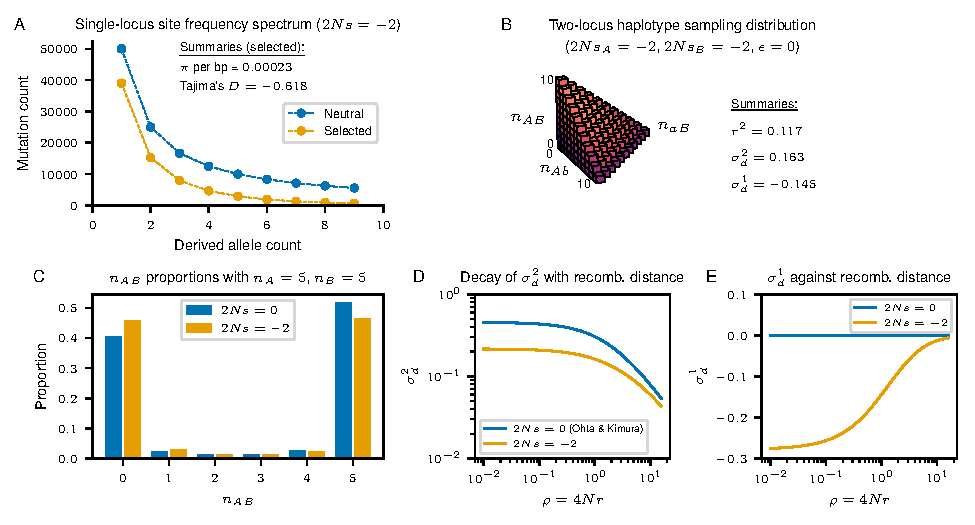
\includegraphics{../figures/two-locus-spectrum/stats_summaries}
    \caption{
        \textbf{Sampling distributions and their summaries.}
        Low-order summaries of sampling distributions are commonly computed
        for allele frequencies (A, the site-frequency spectrum, SFS)
        and two-locus haplotype distributions (B, linkage disequilibrium, LD).
        Demographic and selective processes affect both the SFS and LD,
        and observations of nonzero values of Tajima's $D$ or signed LD
        ($\sigma_d^1$) are often taken as evidence for selection or interactions
        between loci, respectively.
        (C) The full two-locus haplotype sampling distribution is a three-dimensional
        object, making it difficult to visualize. We can instead visualize conditional
        distributions of the full sampling distribution, e.g. conditioned on observing
        five copies of the $A$ allele at the left locus and five copies of $B$ at the
        right locus \citep[e.g.][]{Hudson2001-sg}.
        (D) $\sigma_d^2$, which is closely related to $r^2$, is expected to decay
        with increasing recombination distance between loci \citep{Ohta1969-ie}.
        Selection distorts the level of squared LD away from neutral expectations.
        (E) $\sigma_d^1$, refered to as signed LD here, is expected to be zero for
        pairs of neutral mutations \citep{Hill1968-vu}. Interference between linked
        selected mutation causes negative signed LD \citep{Hill1966-gv}, and other
        forms of interactions between selected mutations can cause large negative
        or positive signed LD.
    }
    \label{fig:TwoLocusFS}
\end{figure}

In the Methods, I expand on the moments system developed in
\citet{Ragsdale2019-nt} to compute the expected sampling distribution
\(\Psi_n\) (Figure~\ref{fig:TwoLocusFS}) of two-locus haplotypes under a
general model of selective interactions. This sampling distribution stores the
expected density or observed counts of pairs of biallelic loci with each
possible haplotype frequency configuration in a sample of size \(n\). Below, we
compute expectations for \(\Psi_n\) under varying scenarios of selection and
interaction between pairs of loci. It is not possible in this framework to
include the effects of additional linked selected mutations, such as background
selection due to many linked variants, and individual-based forward simulations
are still needed for such scenarios (e.g.,
Figures~\ref{fig:bgs1}--\ref{fig:bgs4}).

In many cases it is simpler to visualize summaries such as the expectation or
variance of \(D\) (Figure~\ref{fig:TwoLocusFS}D, E) or conditional slices of the
distribution (Figure~\ref{fig:TwoLocusFS}C) instead of the full
three-dimensional distribution. Here I focus on low-order LD statistics
including \(\E[D]\) and \(\E[D^2]\) and their decay with recombination
distance, as these are statistics that are commonly used to test for
interactions between loci. For pairs of biallelic loci, with alleles labeled
\(A/a\) at the left locus and \(B/b\) at the right locus, \(D=f_{AB}-f_A f_B\)
is the standard covariance measure of LD, where \(f_{AB}\) is the frequency of
haplotypes carrying both \(A\) and \(B\), and \(f_A\) and \(f_B\) are the
marginal allele frequencies of \(A\) and \(B\).

Instead of unnormalized \(\E[D^2]\) and \(\E[D]\) I consider expectations for
\(\sigma_d^2 = \E[D^2]/\E[f_A(1-f_A)f_B(1-f_B)]\) and \(\sigma_d^1 =
\E[D]/\E[f_A(1-f_A)f_B(1-f_B)]\).  Such normalized statistics have two
benefits: first, the mutation rate cancels so that expectations are robust to
assumptions about the per-base mutation rate, and second, we can compare to
analytic expectations for these quantities under neutrality and constant
population size \citep{Ohta1971-yd}.

Below, I first consider the case of additive selection, Hill-Robertson
interference, and epistasis. I then explore the effect of dominance acting
within loci but without epistatis, and then describe a general diploid
selection model and consider gene-based dominance effects. In what follows I
focus on parameters where the strengths of selection and dominance at each
locus are equal, but note that the methods presented here allow for arbitrary
and unequal selection and dominance at the two loci. I also focus primarily on
weak to moderate negative selection (\(|2Ns| \approx 1 - 20\)), since this
range of selection leads to the strongest signals of interference
(Figure~\ref{fig:HillRobertson}) and is the parameter regime for which the
numerical appraoch is most accurate.

\subsubsection{Additive selection and epistasis}
\label{sec:additive-selection}

\begin{figure}[tb!]
    \centering
    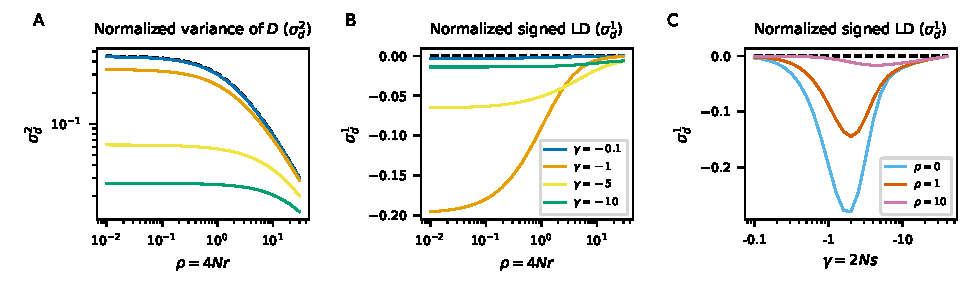
\includegraphics{../figures/hill_robertson}
    \caption{
        \textbf{Hill-Robertson interference.}
        Interference between pairs of selected mutations can cause deviations
        from expected patterns of LD under neutrality, without dominance
        or epistatic effects.
        (A) The expected normalized variance of $D$ (\(\sigma_d^2\))
        decreases below neutral expectations
        as the strength of negative selection increases.
        (B, C) For tightly linked loci (\(4Nr \lesssim 1\)), interference is most
        noticeable as measured by signed LD for pairs of mutations with
        \(s \approx 1/N\).
        At larger recombination distances (\(4Nr > 1\)), signed LD is most
        negative for somewhat stronger selection coefficients.
        Dashed lines show neutral expectations.
    }
    \label{fig:HillRobertson}
\end{figure}

\begin{figure}[tb!]
    \centering
    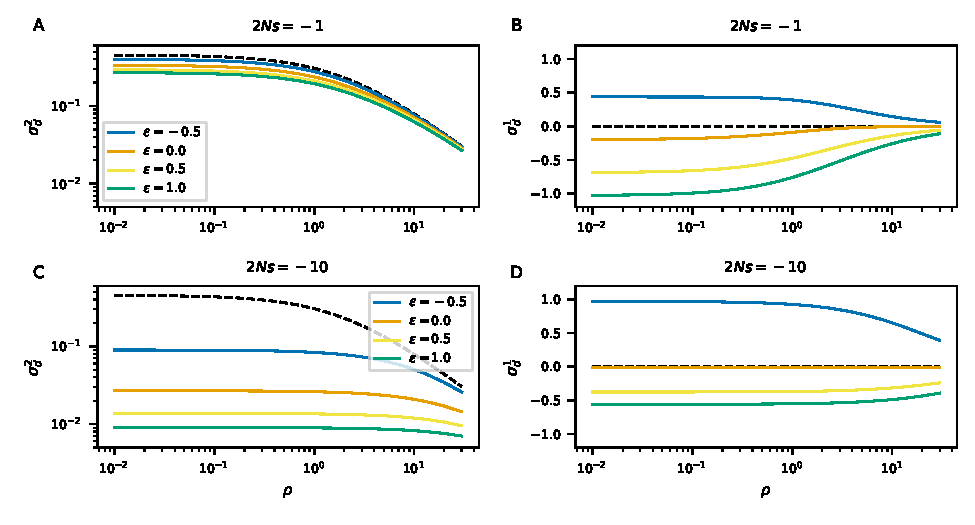
\includegraphics{../figures/epistasis_prediction}
    \caption{
        \textbf{Additive selection and epistasis.}
        Left panels (A and C) show expectations for the decay of
        \(\sigma_d^2 = \E[D^2] / \E[p(1-p)q(1-q)]\) with recombination
        distance, and right panesl (B and D) show expectations for the
        decay of \(\sigma_d^1 = \E[D] / \E[p(1-p)q(1-q)]\). Dashed lines
        show neutral expectations.
        For both weak (\(s=-1/2N\), A and B) and moderate
        (\(s=-10/2N\), C and D) selection,
        antagonistic epistasis (\(\epsilon < 0\))
        gives rise to positive signed LD and increased $\sigma_d^2$ over
        a multiplicative model (\(\epsilon = 0\)),
        and synergistic epistasis (\(\epsilon > 0\)) results in negative signed
        LD beyond that of Hill-Robertson interference and decreased \(\sigma_d^2\).
    }
    \label{fig:epistasis}
\end{figure}

For mutations under additive selection (\(h=1/2\)) and no epistasis, we
recover the well known \citet{Hill1966-gv} interference result of negative LD
between selected mutations, which is strongest for pairs of mutations that have
selection coefficients \(\gamma = O(1)\), or \(s \approx 1/2N_e\) (Figure
\ref{fig:HillRobertson}).
For strongly deleterious mutations, LD is close to zero even
with tight linkage, as they almost always segregate at low enough frequencies
that they are unlikely to interfere with each other \citep{McVean2000-ox}.

With epistasis, mean signed LD is large for both weakly and strongly selected
variants, with sign depending on the direction of epistatic interactions
(Figure \ref{fig:epistasis}).
Synergistic epistasis (in which the effect of two mutations together is larger than
the product of each individual mutation's effect) results in negative LD while
antagonistic epistasis (in which the combined effect is less than the product of
independent effects) results in positive LD, and large positive LD can occur
even when the epistatic effect is relatively weak. Epistasis-induced LD can
extend over long distances, especially for strongly deleterious mutations. For
example, in Figure \ref{fig:epistasis}F even moderately deleterious mutations with
population-size-scaled selection coefficients of \(\gamma=-10\) show large mean
LD that extends to values of \(\rho\) much greater than 1 (for humans, assuming
roughly 1 cM/Mb, this is on the order of 100 kilobases or more).
More strongly deleterious interacting mutations are expected to show large
signed LD over much larger recombination distances.

\subsubsection{Dominance}\label{sec:dominance}

\begin{figure}[tb!]
    \centering
    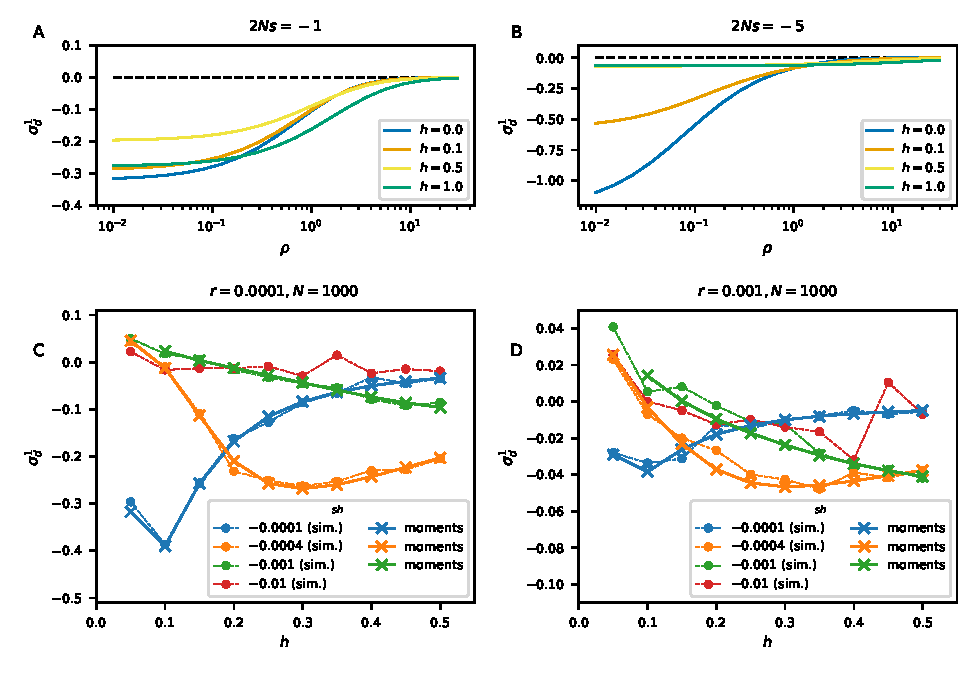
\includegraphics{../figures/dominance_roze}
    \caption{
        \textbf{The effect of dominance on LD.}
        (A, B) The strengths of selection and dominance interact in a nonlinear way
        to shape expected signed LD. For weakly to moderately selected mutations,
        as shown here, signed LD can be large and negative for tightly linked loci
        (e.g., \(\gamma=-5\), \(h=0\), and \(\rho < 1\)). However, this large signed
        LD decays with recombination distance faster under a model of recessivity
        than does signed LD under a model of additive selection and
        epistasis (Figure~\ref{fig:epistasis}).
        (C) Interference effects are most pronounced for recessive deleterious
        variants.
        (D, E) Recessive strongly deleterious mutations can have positive signed
        LD, as recently shown by \citet{Roze2021-cf}.
        However the dominance threshold at which \(\sigma_d^1\) switches from
        positive to negative depends on the strength of selection, and weakly
        selected mutations can show non-monotonic behavior as $h$ varies.
        Selection parameters of \(sh=-0.1\) imply extremely strong selection
        (\(h=0.05\) results in \(s=-0.2\) and \(\gamma=-400\) for homozygous
        diploids at a single locus). The numerical appraoch for \(\Psi_n\)
        cannot handle such strong selection.
    }
    \label{fig:dominance}
\end{figure}

The effect of non-additive selection on correlations between mutations has
received increased attention recently. For example, \citet{Garcia2021-zn} used
large-scale forward simulations to explore how dominance impacts patterns of
LD, showing that LD depends on the magnitudes of both the selection and
dominance coefficients in a nonlinear way. \citet{Roze2021-cf} found an
analytic expression for LD between pairs of strongly deleterious mutations
under steady-state demography, showing that LD can be either positive or
negative depending on the strength of dominance.

The combined effect of the strength of selection and dominance on interference
is indeed nontrivial (Figure~\ref{fig:dominance}A), as observed by
\citet{Garcia2021-zn}. Some parameter regimes can cause strong negative LD
between pairs of negatively selected variants, with moderately selected
recessive variants having stronger signals of interference than additive
selection (Figure~\ref{fig:dominance}B). Unlike epistatic interactions, signed
LD decays rapidly with increasing distance between loci and is roughly zero for
\(\rho \gg 1\). For weakly selected mutations with \(\gamma=-1\), there is no
monotonic effect of the level of dominance on negative LD, with both recessive
and dominant pairs of mutations having more negative LD than the additive case.

Discrete simulations and the moments approach confirm the result from
\citet{Roze2021-cf}, that positive LD can occur for strong negative selection
and small values of \(h\) (Figure~\ref{fig:dominance}D, E). However, while the
analytic formula in \citet{Roze2021-cf} predicts that LD should be positive for
\(h<0.25\) and negative for \(h>0.25\), this appears to only hold in the limit
of strong selection (compare to Figure 1A in \citet{Roze2021-cf}). For moderate
to moderately strong selection, this threshold of \(h\) can be less than
\(0.25\), and LD is negative for all \(0\leq h \leq 1\) for weakly deleterious
mutations with interference strongest between pairs of recessive mutations
(Figure~\ref{fig:dominance}C).

\subsubsection{General selection and gene-based dominance}
\label{sec:general-selection}

\begin{figure}[tb!]
    \centering
    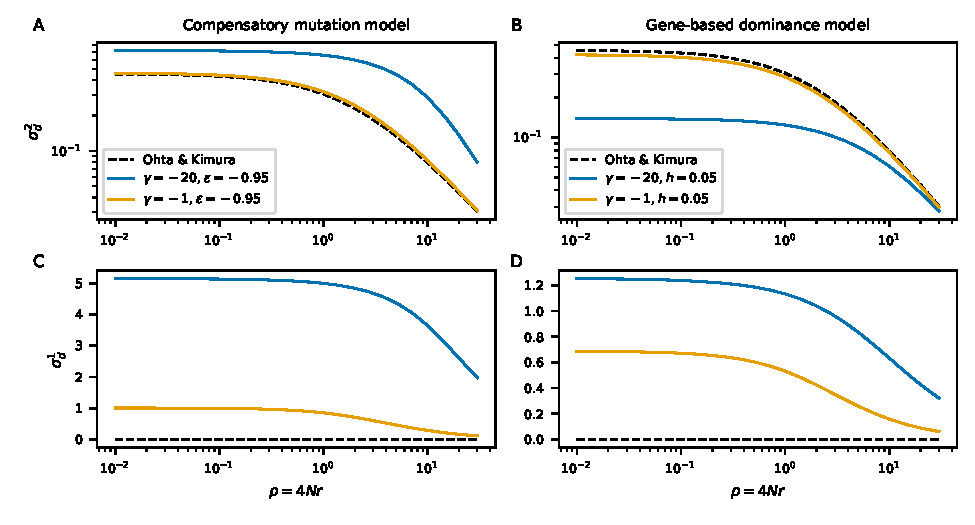
\includegraphics{../figures/gene-based-compensatory}
    \caption{
        \textbf{Multiple modes of interactions can lead to large positive signed LD.}
        Both antagonistic epistasis (A and C, and which includes compensatory mutation
        models) and gene-based dominance (B and D) lead to large positive signed LD.
        Compensatory mutations (\(\epsilon \approx -1\)) also cause increased
        \(\sigma_d^2\) compared to neutral expectations (dashed black lines),
        while weaker antagonistic epistasis does not increase \(\sigma_d^2\) above
        neutral expectations (compare to Figure~\ref{fig:epistasis}C).
        Gene-based dominance instead causes lower \(\sigma_d^2\) than neutral
        expectations.
        While signed LD may be similar between different interaction models,
        other two-locus summaries of the data may help to distinguish between
        such models.
        }
    \label{fig:gene-based-compensatory}
\end{figure}

Beyond the standard models of epistasis and dominance shown above, a large
family of selection models can be specified by assigning unique fitness effects
to each possible diploid pair of haplotypes. If we assume the diploid genotype
that is homozygous for the ancestral alleles (\(ab/ab\)) has fitness 1, then
there are nine other possible diploid two-locus genotypes that could be given
unique fitnesses (Table \ref{tab:selmodels}), noting that \(AB/ab\) and
\(Ab/aB\) genotypes can have differing selection coefficients.

The case with \(s_{AB/ab} \not= s_{Ab/aB}\) arises in a scenario where a
mutation at either locus within a haplotype impacts some functional region or
element, but a diploid individual carrying at least one copy that is free of
mutations has minimal fitness loss. In this ``gene-based dominance'' scenario
\citep[e.g.,][]{Sanjak2017-zw}, an \(AB/ab\) genotype has higher fitness than
an \(Ab/aB\) type (a simple implementation of this model is given in the final
column in Table \ref{tab:selmodels}). Such a gene-based fitness model gives
similar expected positive signed LD to the model of antagonistic epistasis
(Figure~\ref{fig:gene-based-compensatory}), although the interpretation of
those two models can differ. With a highly parameterized space of possible
general diploid selection models, multiple models with different biological
interpretations can give similar patterns of expected signed LD.

\subsection{The effect of population size changes on signed LD}
\label{sec:demography}

\begin{figure}[tb!]
    \centering
    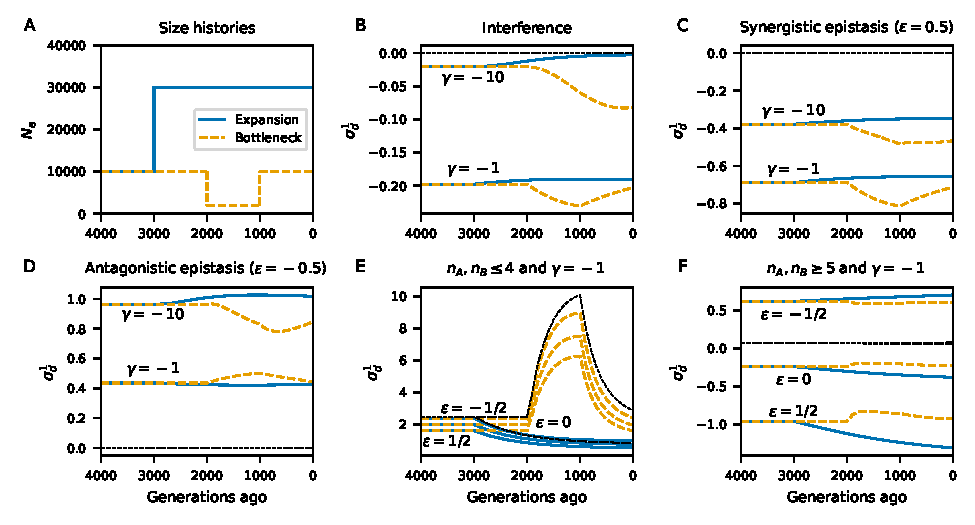
\includegraphics{../figures/demog_bottle_expand}
    \caption{
        \textbf{The effects of demography on signed LD.}
        Simulations under two toy models, one with an instantaneous expansion in
        the past and the other with a five-fold reduction and recovery illustrated
        in (A), show the effects of population size changes on expected patterns of LD. 
        For two selection strengths (\(\gamma=-1\) and \(\gamma=-10\)) and three
        cases of interactions (non-epistatic interference (\(\epsilon=0\), B),
        synergistic epistasis (\(\epsilon=1/2\), C), and antagonistic epistasis
        (\(\epsilon=-1/2\), D), each with \(\rho=0\)),
        sudden decreases in population size can cause
        large changes in signed LD, often in the opposite direction than more
        subtle shifts due to instantaneous expansion events.
        (E) Signed LD between pairs of rare alleles (both \(n_A, n_B \leq 4\), with
        sample size \(n=50\)) is more sensitive to population size changes.
        (F) Signed LD between pairs of common alleles (both \(n_A, n_B \geq 5/50\))
        is comparatively more stable over time.
        Additional comparisons, including for dominance models and showing
        \(\sigma_d^2\), are shown in Figures~\ref{fig:toy_sd2}--\ref{fig:toy_dom_sd2}.
        Dashed lines indicate neutral expectations.
    }
    \label{fig:toy}
\end{figure}

\begin{figure}[tb!]
    \centering
    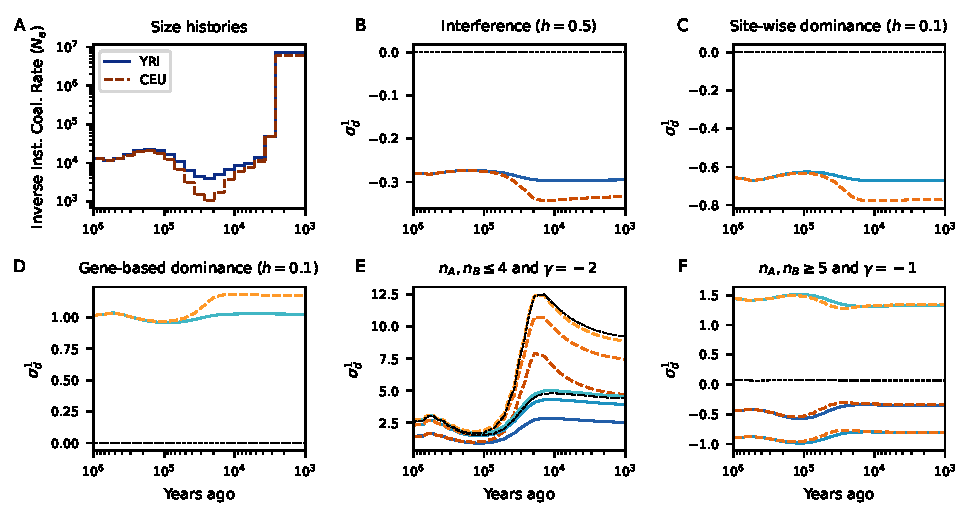
\includegraphics{../figures/demog_YRI_CEU.dominance}
    \caption{
        \textbf{Signed LD under inferred models of human population-size history.}
        Piecewise-constant population size histories inferred by Relate applied to
        \citet{1000_Genomes_Project_Consortium2015-zq} phase 3 data were used to
        simulate time series of two-locus statistics, as in Figure~\ref{fig:toy}.
        (A) The CEU (Utah residents with Northern and Western European ancestry)
        are inferred to have a stronger bottleneck than the YRI
        (Yoruba in Ibadan, Nigeria) 10--100ka, reflecting the out-of-Africa
        event.
        Here, we highlight the effect of size changes on \(\sigma_d^1\) under
        non-additive selection models with \(\rho=0\) and \(\gamma=-2\) at both loci,
        comparing standard interference (B) to site-wise dominance (C) and gene-based
        dominance (C).
        As with epistasis, more severe bottlenecks have larger effects on signed LD,
        and LD among common variants is more stable than among pairs of rare variants.
        Additional comparisons with epistasis and showing \(\sigma_d^2\) are
        in Figures~\ref{fig:relate}--\ref{fig:relate_dom_sd2}.
        Dashed lines indicate neutral expectations.
    }
    \label{fig:relate_dom}
\end{figure}

The moment system for \(\Psi_n\) readily incorporates variable population size as
well as mutation and recombination rates and selection parameters that change
over time. Here I focus on non-equilibrium population size history and consider
scenarios relevant to human demographic history, including bottlenecks and
expansions. I explore two simple models (Figure \ref{fig:toy}A), one with an
instantaneous expansion and another with a bottleneck followed by recovery. I
also consider two demographic histories inferred using genome-wide gene
genealogy reconstruction \citep{Speidel2019-nj} applied to the
\citet{1000_Genomes_Project_Consortium2015-zq} dataset, and focus on size histories
for the Yoruba from Ibidan, Nigeria (YRI) and Utahns of North and West European
ancestry (CEU) (Figure \ref{fig:relate_dom}B).

For each of the four histories,
Figures~\ref{fig:toy},~\ref{fig:relate_dom},~and~\ref{fig:toy_sd2}--\ref{fig:relate_dom_sd2}
show the dynamics of \(\sigma_d^1\) and \(\sigma_d^2\) for a given
parameterization of two-locus selection, including synergistic and antagonistic
epistasis, dominance within loci, and gene-based dominance. In general across
each selection model, population size expansions are not expected to strongly
affect \(\sigma_d^1\), whether that expansion occurs deeper in the past as in
the simple expansion model or rapid expansion more recently, as in the YRI. On
the other hand, population size reductions tend to push signed LD to more
extreme values and subsequent recoveries or expansion again reduce the
magnitude of LD. Under no selection condition tested here do population size
changes cause expected LD to change sign, showing that while the magnitude of
deviation of LD from zero is sensitive to population size history, interpreting
general patterns of the observed sign of LD in data should not be strongly
affected by population size history.

\subsection{Signed LD within protein-coding genes}

\begin{figure}[tb!]
    \centering
    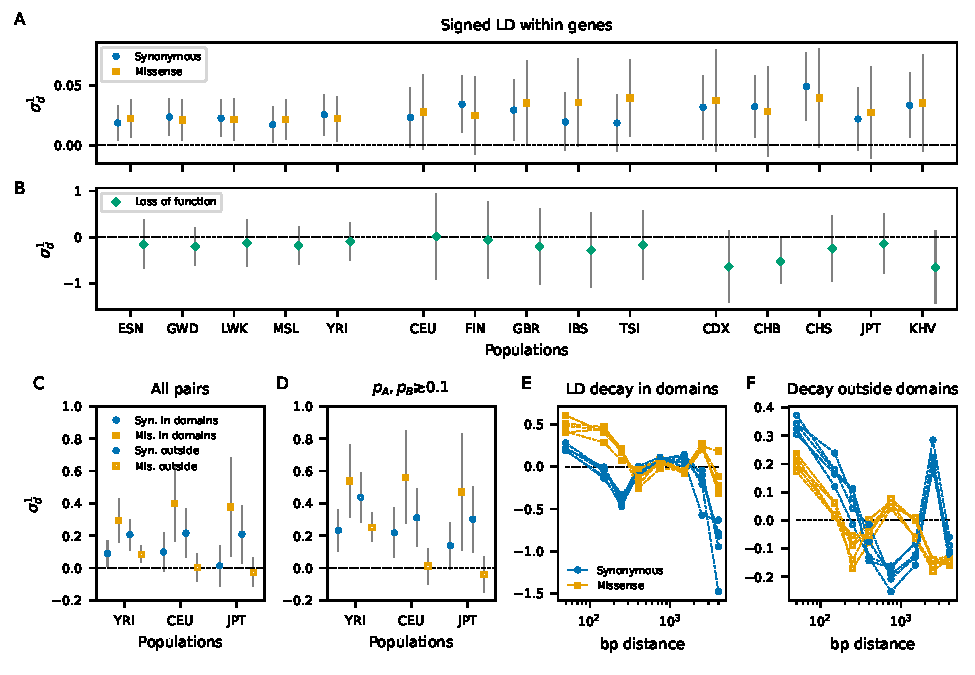
\includegraphics{../figures/data_compact}
    \caption{
        \textbf{LD in human protein-coding genes and annotated domains.}
        (A) Gene-wide averages of signed LD are slightly positive between pairs
        of both missense and synonymous mutations, considering pairs of mutations
        at matching distances. This positive, equal \(\sigma_d^1\) is also observed
        when conditioning on allele frequencies or considering only common variants
        with minor allele frequencies \(\gtrsim 0.1\)
        (Tables~\ref{tab:afrsd1}--\ref{tab:eassd2}).
        (B) While there are relatively fewer pairs of loss-of-function mutations
        within genes, causing larger measurement uncertainty, such pairs tend to have
        negative average LD. Note that measurement noises for each class of
        mutations overlap with zero and with each other, making it difficult to
        draw firm conclusions on the patterns of interactions occurring gene-wide.
        (C) Partitioning pairs of mutations as falling within or outside
        of conserved domains reveals opposing patterns of signed LD, with
        \(\sigma_d^1\) between missense mutations larger than that of synonymous
        mutations within domains. Outside of conserved domains, missense mutations
        have reduced LD compared to synonymous mutations. Distances of pairs outside
        of domains were matched to within-domain mutation pair distances.
        (D) This pattern again holds for common variants.
        (E, F) The signal of increased LD between missense variants within domains
        and decreased LD outside of domains is driven largely by tightly linked
        mutations (distances \(\lesssim 400\) bp), here showing African populations
        in the \citet{1000_Genomes_Project_Consortium2015-zq}.
        Additional comparisons are shown in the Supporing Information, and Thousand
        Genomes population labels are described in Table~\ref{tab:1kgpops}.
    }
    \label{fig:data}
\end{figure}

Here, I examine patterns of signed LD between mutations in human protein-coding
genes partitioned by functional annotations. Synonymous and missense mutations
show similar levels of slighly positive signed LD when considering pairs of
mutations within the same gene averaged over all autosomal chromosomes.
Loss-of-function mutations have more negative LD, possibly suggesting differing
modes of selective interactions for loss-of-function and missense mutations
(Figure \ref{fig:data}A--B). Within each population, measurement noise gives
95\% confidence intervals that overlap with zero in each mutation class,
although the observed patterns are remarkably consistent across African,
European, and East Asian populations in the Thousand Genomes dataset. Comparing
mean LD across populations, LD in Eurasian populations is somewhat larger on
average, that is, more positive for missense mutations and more negative for
loss-of-function mutations. This is in agreement with differences in
expectations between populations that have or have not gone through a
bottleneck in their recent history
(Figures~\ref{fig:toy}~and~\ref{fig:relate_dom}).

\subsubsection{Positive LD between pairs of missense mutations in conserved domains}

The similarity in signed LD between missense and synonymous mutations would
suggest that interference between missense mutations is minimal, or at least no
stronger than interference between synonymous mutations. However, interactive
effects differ dramatically between pairs of mutations found in different
intra-genic regions, with opposing effects canceling out when taking gene-wide
averages. Due to the rarity of loss-of-function mutations, I only compare
synonymous and missense mutations when looking at finer partitions of mutations
within genes.

Annotated conserved domains in protein-coding genes play a significant role in
driving signals of positive LD within genes. Such protein-coding domains are
conserved elements of genes, often associated with some known functional or
structural feature of a protein \citep{Stanek2020-pa}. Purifying selection is
expected to be stronger within conserved domains than within the same gene but
outside of those domains. Indeed, the site-frequency spectrum (SFS) is skewed
to lower frequencies for both missense and loss-of-function mutations within
domains when compared to the same classes of mutations outside of domains, with
much more negative values of Tajima's D within domains (Table
\ref{tab:tajimasD}). On the other hand, no difference is observed for
synonymous mutations whether within or outside domains, suggesting roughly
equivalent effects of selection (either direct or linked) on synonymous
variation.

Pairs of missense mutations that both fall within the same functional domain
have large positive LD that is elevated above that of pairs of synonymous
mutations that both fall within the same domain
(Figures~\ref{fig:data}C--F~and~\ref{fig:LDwithin}--\ref{fig:domainsEAS}). This
difference between pairs of missense and synonymous variants within domains is
especially pronounced for linked pairs within a few hundred base pairs of each
other (Figures~\ref{fig:data}E~and~\ref{fig:LDwithin}). Assuming most
synonymous mutations are neutral, we would expect signed LD between missense
mutations to be less than that between synonymous mutations under predictions
from models of either Hill-Robertson interference, synergistic epistasis, and
some models of dominance (Figures~\ref{fig:epistasis}~and~\ref{fig:dominance}).
This observation is opposite to those expectations, suggesting a different
prevailing interactive effect between nonsynonymous mutations within domains.

The strength of selection on missense mutations within and outside of domains
is observed to differ, leading to an excess of rare missense mutations within
conserved domains (Table~\ref{tab:tajimasD}). LD is known to be sensitive to
allele frequencies, with rare mutations showing large positive signed LD
\citep{Good2022-ot}. To test whether the signal of increased LD between
missense mutations within domains is driven by rare variants, I considered
subsets of pairs of mutations based on their derived allele frequences
(Figures~\ref{fig:data}D~and~\ref{fig:domainsAFR}--\ref{fig:domainsEAS}). Rare
and uncommon variants show large average LD for each class of mutations, but
common variants recapitulate the opposing patterns of LD that is seen when
averaging over pairs at all frequencies, as unconditioned statistics in the
form of \(\sigma_d^1\) and \(\sigma_d^2\) are dominated by common variants.

\subsubsection{Reduced LD between pairs of missense mutations outside of conserved domains}

The large positive signal of LD for missense mutations within the same domain
does not extend to pairs of missense mutations that are in different domains.
Pairs of missense and synonymous mutations show nearly equal levels of LD close
to zero across domains, with missense mutations slightly more negative than
synonymous mutations (Figure \ref{fig:between_domains}). The interactive effect
driving large LD in domains is therefore likely domain-specific. However, the
average distance between pairs of mutations within domains is much smaller than
between domains, and this observation may be primarily driven by the higher
recombination distances between pairs of mutations across distinct domains.

Pairs of mutations that both fall outside of annotated domains have the
opposite pattern of signed LD to pairs of mutations falling within the same
domain. For pairs of mutations outside of domains but with distances matched to
those within domains, pairs of synonymous mutations have larger positive LD
than missense mutations. More distant pairs of mutations outside of domains,
matched to the same distances as the between-domain comparison, each have LD
roughly equal to zero (Figure~\ref{fig:between_domains}).

The role that tightly linked variants have in driving these opposing signals
can be seen in the decay of signed LD with distance between mutations
(Figures~\ref{fig:LDgene}--\ref{fig:LDoutside}). Both synonymous and missense
mutation pairs at distances greater than a few hundred base pairs have average
LD that fluctuates around zero. However, for mutations outside domains,
synonymous variants separated by short distances have large positive LD, while
missense mutations have lower LD (Figure~\ref{fig:LDoutside}). In contrast, for
mutations within the same domains, missense mutations have more positive LD at
short distances than synonymous mutations (Figure~\ref{fig:LDwithin}).

\section{Discussion}\label{sec:discussion}

Previous theoretical and simulation studies have shown that interference and
interactions between selected mutations reduce the efficacy of selection at
linked loci, impacting substitution rates, the deleterious mutation load, and
dynamics of segregating mutations
\citep{Hill1968-vu,Birky1988-jm,Barton1995-mj,McVean2000-ox}. Interference and
synergistic epistasis between moderately deleterious mutations are both
expected to cause negative LD between selected mutations, which can be readily
tested using population genetic data
\citep{Sohail2017-zq,Sandler2021-of,Garcia2021-zn}. Here, I used a closed
numerical approach to generate expectations for LD under a wide range of
selective scenarios, and then compared patterns of LD in human populations
between classes of coding mutations using unbiased estimators for LD from
unphased genotypes.

By taking broad genome- and gene-wide surveys of LD across functional classes
of mutations, heterogeneous patterns of interactive effects that occur within
genes can be missed. From gene-wide averages, LD between pairs of missense
mutations does not appear to be different from pairs of synonymous variants,
although LD between loss-of-function variants is more negative. Hill-Robertson
effects are expected to be strongest for slightly to moderately deleterious
variants (with \(|s|\sim 1/N_e\)), as strongly deleterious mutations are not
expected to interfere with one another \citep{McVean2000-ox}. However,
loss-of-function mutations do not typically fall within this regime, and
inference of the distribution of fitness effects (DFE) for new loss-of-function
variants shows that a large majority are strongly deleterious (Supporting
Information).

Instead, negative synergistic epistasis between strongly deleterious mutations
does produce large negative deviations of mean LD. Weakly deleterious
recessive mutations can also produce this pattern, but strongly deleterious
recessive mutations lead to slightly positive LD \citep{Roze2021-cf}. While
most loss-of-function mutations are strongly deleterious, those that rise to
appreciable frequency are likely more benign and \(\sigma_d^1\) may be driven
by patterns of weakly deleterious loss-of-function mutations. The difficulty in
distinguishing these effects is compounded by the large measurement noise for
\(\E[D]\), especially for loss-of-function variants for which only a few
hundred within-gene pairs exist in the human population data analyzed here and
which are separated by larger distances on average than neighboring missense
and synonymous mutations.

In addition to LD varying by distance, LD can also vary due to differences in
allele frequencies among classes of mutations (as selection drives mutations to
higher or lower frequencies). Matching distances between pairs as well as
allele frequecies between classes of mutations helps to reduce these concerns.
It is possible that recombination rates can vary between annotated regions,
resulting in differing patterns of background selection, which can affect
allele frequencies and LD (e.g., Figures~\ref{fig:bgs1}--\ref{fig:bgs4}). I did
not condition on local recombination rates or inferred levels of background
selection here, which is left to future work.

\subsection{Non-uniform interactions between selected mutations within genes}

Positive average LD between both missense and synonymous mutations has been
reported in humans, \emph{Drosophila}, and other species
\citep{Sohail2017-zq,Sandler2021-of}, while others have found that
nonsynonymous mutations show lower LD than synonymous mutations
\citep{Garcia2021-zn}. The similarity of their gene-wide LD observed in this
study (Figure~\ref{fig:data}) might suggest that interference or interactions
between missense mutations are minimal, or at least no stronger than those
between synonymous mutations. However, averaging over all observed pairs of
mutations within a gene masks element-specific interactive effects that drive
LD in opposite directions. Nonsynonymous mutations found within conserved
protein domains, identified as conserved subunits of a gene with some
structural or functional role \citep{Stanek2020-pa}, are more strongly selected
against on average, but also have increased signed LD over synonymous mutations
at the same distances within domains. Missense mutation outside of domains but
at the same distances as those within domains have more negative LD, both
compared to distance-matched synonymous mutations outside of domains and to
mutations within domains.  Neither dominance effects (aside from very strongly
selected recessive mutations \citep{Roze2021-cf}), synergistic epistasis, nor
Hill-Robertson interference are expected to result in positive LD, so some
other interactive effect should be driving this signal of positive LD within
conserved domains.

There are a number of possible interaction scenarios that can result in
positive signed LD between tightly linked loci. One explanation is a prevalence
of pairs of compensatory mutations that are tolerated to co-segregate at high
frequencies within conserved domains \citep{Yeang2007-gj,Ivankov2014-tn}.
\citet{Callahan2011-ac} and \citet{Taverner2020-lk} have proposed such a
mechanism to explain observed clusters of nonsynonymous mutations in lineages
of \emph{Drosophila} and other species. Another possibility is a model of
antagonistic, or diminishing returns epistasis, in which a single amino
acid-changing mutation within a domain damages the functionality of that
subunit, but additional mutations within that same domain reduce fitness by a
factor less than the first mutation. A third possibility, related to
antagonistic epistasis, is that selection acts on the functional domain as a
unit instead of on mutations within the domain individually (such as under a
model of gene-based dominance). In this scenario, double heterozygotes have
different fitnesses depending on whether the mutations are found on same
haplotype or on different haplotypes.

We do not see an increase in LD between mutations that are found in different
annotated domains within the same gene, which are on average at much larger
recombination distances. Nor do we find increased LD outside of domains.
Rather, for pairs of mutations outside of domains but matched to the same
distance as those within the same domain, missense variants have considerably
lower LD than synonymous variants. This difference between synonymous and
missense pairs of variants largely disappears for SNPs separated by more than a
few hundred base pairs (Figure~\ref{fig:data}E, F). This suggests that
Hill-Robertson interference is the primary mode of interaction between missense
mutations falling outside of domains, in agreement with \citet{Garcia2021-zn},
as epistasis is expected to impact LD over larger distances than what is
observed. Importantly, however, the strength of epistasis is also likely to be
a function of distance between mutations, complicating this interpretation.

Taken together, selection on segregating variants within protein-coding genes
is nonuniform, with both the overall strength of selection and interactions
between variants differing between annotated elements. Missense and
loss-of-function mutations within conserved domains are subject to stronger
selection, skewing the SFS to lower frequencies. Typical approaches for
inferring the distribution of fitness effects from population genomic data
average over these differences by considering all nonsynonymous mutations
together \citep{Boyko2008-zk,Kim2017-xo}. If patterns of selection differ by
both mutational class and location or if loss-of-function variants are in fact
recessive, this can impact inferences of the DFE (Supporting Information). It
would be straightforward to adapt DFE-inference methods to infer more detailed
representation of the heterogeneous effects of new mutations within genes by
partitioning by missense and loss-of-function classes as well as by annotated
domains. Similarly, the different modes of interaction between mutations across
annotated domains mean that our standard models and simulation approaches may
be too simple to capture the evolutionary trajectories and patterns of
diversity that differ at finer scales.

\subsection{Clustered mutations may cause positive LD among synonymous mutations}

In a non-structured randomly mating population, neutral mutations are expected to have
average signed LD of zero, but across all populations analyzed here, LD between
synonymous mutations is positive. While selection on some subset of synonymous
variants is possible, it should be much weaker on average than between missense
mutations, and any interference between selected synonymous variants should
lead to negative LD.

Spatial population structure may be responsible for the increase of LD observed
between synonymous variants. Neutral evolution in structured populations alone
cannot create this effect. Under standard population genetic assumptions of
constant mutation and recombination rates and independent mutation events,
migration, admixture, and spatial structure do not result in nonzero \(\E[D]\).
Rather, for a set of mutations with \emph{given} differences in allele
frequencies between source populations, \(D\) can be nonzero in an admixed
population between those particular mutations even when \(D\) is zero in the
source populations \citep{Cavalli-Sforza1971-jv}. This result relies on
conditioning on directional differences in allele frequencies between
populations. Without conditioning, the expected difference in mean allele
frequency between source populations is zero (\(\E[(p_1-p_2)(q_1-q_2)] = 0\)),
as differences are equally likely to be positive or negative, and thus
resulting \(\E[D]\) is still zero when taking genome-wide averages.

Instead, \citet{Sohail2017-zq} and \citet{Sandler2021-of} used forward
simulations under multi-population or explicit spatial models and a
multiplicative fitness function to explore the joint effects of structure,
assortative mating, and interference, finding that together these can lead to
nonzero LD. For example, \citet{Sandler2021-of} found positive LD among neutral
mutations in a simulation with admixture and linked selected mutations, showing
that the combined effects of spatial structure and background selection can
lead to positive average LD between neutral mutations. Positive LD between
synonymous mutations is only observed at short distances in human data, which
could be used to constrain such models that predict positive LD over varying
distances.

Nonrandom mutational processes provide an alternative explanation for positive
LD between neutral variants separated by short distances, in which clusters of
mutations occur simultaneously in the same mutational event. Such
multinucleotide mutations have been shown to affect patterns of LD over short
distances, on the order of 10s to 100s of base pairs \citep{Harris2014-zg}, and
clustered mutational events may be common in humans \citep{Besenbacher2016-ac}.
Indeed, a simple exponential model in which the fraction of pairs of mutations
arising from a multinucleotide mutation event decays with distance fits the
observed decay of \(\sigma_d^1\) between synonymous variants (Supporting
Information, Figure~\ref{fig:mslmnms}), with the best-fit model requiring only
a small fraction of mutations to cause multinucleotide mutation events. We may
therefore treat positive LD as the baseline expectation for tightly linked
variants primarily due to clustered mutations, so that subsequent selective
processes and interactions cause LD to deviate from that expectation, as seen
for missense mutations across different sub-elements of genes. It may also be
more appropriate to compare the negative LD observed between linked
loss-of-function variants to that positive baseline expectation instead of
zero, which would imply that they are more recessive or have stronger
synergistic epistasis than from inferences assuming a neutral expectation of
zero. Additional analyses and extensive simulations will be required to tease
apart the effects of population structure, selective interference at linked
sites, and clustered mutational events on patterns of LD.

\subsection{Challenges to distinguishing highly parameterized models of selective interactions}

When partitioning measurements of LD by mutation classes or regions within
genes, the decreasing number of pairwise comparisons leads to large estimated
measurement noise. Within each population, confidence intervals of observed
\(\sigma_d^1\) often overlap with zero or overlap with that of other classes of
mutations. While observed patterns are remarkably consistent across the 15
populations considered here, their joint evolutionary histories make formal
testing of significance difficult due to shared variation, as they cannot be
treated as independent measurements. Extensive forward simulations will likely
be needed to more thoroughly assess significance.

From a modeling perspective, in exploring or inferring multi-locus selective
models, the number of plausible selection scenarios becomes quite large as we
relax the strict assumptions of additivity and multiplicative fitness effects.
The inclusion of dominance effects, epistasis, or other interactions leads to a
rapid increase in the number of parameters to consider. This makes performing
forward simulations that span the range of all such selective interaction
scenarios burdensome. 

Instead, closed, numerical approaches to compute expectations for two-locus
statistics under a wide range of selection models, as presented here and in
\citet{Friedlander2022-bs}, allow us to explore this highly parameterized space
of models far more efficiently, and it opens the possibility for performing
likelihood-based inference using signed LD or other two-locus summaries of the
data. For example, inferring the joint distribution of dominance and selection
is underpowered using the SFS alone, but because signed LD is sensitive to the
levels of dominance (Figure~\ref{fig:dominance}), inferring the DFE with
dominance may be feasible using the joint distribution of allele frequencies
and LD. The results presented in this paper likely do not cover the space of
all possible two-locus models, and other unexplored models may result in
similar patterns of signed LD. Comparisons to empirical data should therefore
be treated with caution, and additional careful modeling will allow a more firm
determination of the interactive effects causing observed patterns of
variation.

Using a single low-order summary of signed LD, such as \(\E[D]\) or
\(\sigma_d^1\), is likely insufficient to confidently discriminate modes of
selective interactions between linked mutations. Both dominance and epistasis
can result in strongly negative LD, although the expected decay of LD under
those scenarios can differ. Similarly, multiple interaction models can lead to
positive signed LD. Among all interaction models, the extent of LD and rate of
its decay also depends on the underlying distribution of selection coefficients
among a class of mutations, which are unknown for a given pair of mutations, so
that we must integrate over a distribution of fitness effects. This DFE,
however, will have been inferred under a simple set of assumptions, such as
additivity and interchangeability between sites within a gene, potentially
biasing any inference using previously inferred DFEs to learn about patterns of
interactions. Again, this underlines the need to jointly infer strengths and
interactions of selected variants.

Finally, exploring additional summaries of the two-locus sampling distribution
should provide additional power to distinguish between interaction models. The
numerical methods developed here provide the full two-locus sampling
distribution, and expectations for a large family of informative two-locus
statistics can be computed directly from this distribution. These expectations
can then be compared directly to empirical observations, which can be taken
from either phased or unphased data \citep{Ragsdale2020-nz}. Additional work
performing such an analysis is therefore warranted, which should provide a path
forward for distinguishing between modes of selective interactions.

\section{Methods}\label{sec:methods}

\subsection{Existing theory and numerical methods}

Many well-known properties of two-locus dynamics and equilibrium LD come from
early work on the multi-locus diffusion approximation \citep{Kimura1955-qe,
Hill1968-vu, Ohta1969-ie, Ohta1971-yd}. This includes the result that
genome-wide averages of signed LD are expected to be zero under neutrality.
Under a two-locus biallelic model, where the left locus allows alleles \(A\)
and \(a\) and the right locus allows alleles \(B\) and \(b\), the standard
covariance measure of LD is defined as \(D = f_{AB} - f_{A}f_{B}\), where
\(f_{AB}\) is the haplotype frequency of double-derived types carrying both
\(A\) and \(B\), and \(f_{A}\) and \(f_{B}\) are the marginal frequencies of
the derived alleles at each locus. This covariance decays due to both drift and
recombination at a rate proportional to the inverse of the effective population
size and the distance separating loci \citep{Hill1968-vu}:
\[\E[D]_{t+1} = \left(1 - \frac{1}{2N_e(t)} - r \right)\E[D]_t.\]
While \(\E[D] = 0\), the variance of \(D\) is non-zero, and \citet{Ohta1971-yd}
presented their groundbreaking result that the variance of \(D\) under
neutrality and steady-state demography, normalized by the joint heterozygosity
of the two loci, is
\begin{equation}
    \label{eq:ohta}
    \sigma_d^2 = \frac{\E[D^2]}{\E[f_A(1-f_A)f_B(1-f_B)]}
    \approx\frac{5 + \rho / 2}{11 + 13\rho/ 2 + \rho^2 / 2},
\end{equation}
where \(\rho = 4N_e r\).

Analytic progress beyond these results has come haltingly. In the 1980s,
recursions were developed to compute the two-locus sampling distribution under
neutrality, that is, the probability of observing given counts of two-locus
haplotypes in a sample of size \(n\) \citep{Golding1984-pu}. This approach
would continue to be developed and later form the foundation for the inference
of local recombination rates from population genetic data
\citep{Hudson2001-sg,McVean2004-gj}. More recently, \citet{Song2007-qk}
computed \(\E[r^2]\) using a diffusion approximation approach, although their
solution involves the summation of infinitely many terms and is restricted to
neutrality and steady-state demography.

To include selection, however, there have been relatively few advances beyond
the Monte Carlo simulation approach taken by \citet{Hill1966-gv}, albeit now
with more powerful computational resources and sophisticated software for
performing flexible forward simulation
\citep[e.g.][0]{Thornton2019-qc,Haller2019-vm}. Analytic results for two-locus
distributions under selection are notoriously difficult, with a few notable
flashes of progress. For example, \citet{McVean2007-xd} considered the effect
of a recent sweep on patterns of LD between neutral loci near the locus under
selection, and in a recent paper, \citet{Good2022-ot} presented analytic
solutions for patterns of LD between rare mutations under additive selection
with epistasis. Nonetheless, such approaches are typically confined to
steady-state demography and constrained selection models.

Numerical methods inhabit the space in between expensive discrete simulations
and limited analytic solutions, providing a more efficient and practical method
to compute expectations of two-locus diversity measures under a wider range of
parameters and demographic scenarios. \citet{Ragsdale2017-gg} used a finite
differencing approach to numerically solve the two-locus diffusion equation
with additive selection at either locus, although that paper focused on the
applicability of two-locus statistics to demographic inference. More recently,
\citet{Ragsdale2019-nt} extended the \citet{Hill1968-vu} system for \(\E[D^2]\)
to compute arbitrary moments of the distribution of \(D\) for any number of
populations connected by migration and admixture. They also showed that such a
moments-construction can be used to solve for the two-locus sampling
distribution within a single population, though it requires a moment-closure
approximation for nonzero recombination and selection. Below, I extend this
approach to model arbitrary diploid selection, which encompasses dominance,
epistasis, and other forms of selective interactions between two loci. In a
concurrent study to this paper, \citet{Friedlander2022-bs} developed numerical
solutions to the same moments system, which they used to describe selected
haplotype trajectories and the distortion of neutral diversity at loci variably
linked to beneficial alleles that sweep to high frequencies under
non-equilibrium demography.

\subsection{The two-locus sampling distribution with arbitrary selection}

The two-locus sampling distribution is the direct analog to the single-locus
site frequency spectrum (SFS) of a given sample size
(Figure~\ref{fig:TwoLocusFS}). Instead of describing the density or number of
mutations with a given allele count out of \(n\) samples, the two-locus
distribution \(\Psi_n\) stores the density or number of pairs of loci with
observed haplotype counts, so that \(\Psi_n(i, j, k)\) is the number of pairs
for which we observe \(i\) copies of the \(AB\) haplotype, \(j\) of type
\(Ab\), \(k\) of type \(aB\), and \(n-i-j-k\) of type \(ab\). The size of
\(\Psi_n\) grows rapidly, with \(O(n^3)\) entries, which practically limits
computational approaches to moderate sample sizes \(n\lesssim 100\) and a
single population.

Under neutrality, a number of approaches exist to compute \(\Psi_n\), including
the recursion due to \citet{Golding1984-pu} and \citet{Ethier1990-tb}, or more
recent numerical approaches to the two-locus coalescent \citep{Kamm2016-ag} or
diffusion approximation \citep{Ragsdale2017-gg}. Selection is most easily
included using the forward-in-time diffusion equation
\citep{Kimura1955-qe,Hill1966-gv}, where a standard approach is to first solve
for the continuous distribution \(\psi\) of the density of two-locus haplotype
configurations in the full population, and then integrate \(\psi\) against the
multinomial sampling function to obtain \(\Psi_n\).

Alternatively, \citet{Ragsdale2019-nt} showed that there exists a system of
ordinary differential equations directly on the entries of \(\Psi_n\). I
briefly summarize this general approach below, but refer readers to that paper
for detailed derivations of the drift, recombination, and mutation terms and
the moment-closure approximation. Instead, here I focus on generalizing the
selection operator to include epistasis, dominance, and other forms of
two-locus interactions.

\subsubsection{Moment equation for \(\Psi_n\)}

The system of linear ordinary differential equations for the entries of
\(\Psi_n\) takes the form
\begin{equation}
\label{eq:system}
{\Psi}_n^{t+1}(i, j, k; t) =
\mathcal{D}_{N(t)}\Psi_n^t
+ \mathcal{R}_{r}\Psi_{n+1}^t
+ \mathcal{U}_{u}\Psi_n^t
+ \mathcal{S}_{s_A, s_B, \ldots, h_A, h_B, \ldots}\Psi_{n+2}^t.
\end{equation}
Here, \(\mathcal{D}_{N(t)}\) is a sparse linear operator accounting for drift
with population size \(N(t)\), \(\mathcal{R}\) accounts for recombination
with per-generation recombination probability \(r\) between the two loci,
\(\mathcal{U}\) accounts for mutation, either under an infinite sites or
biallelic reversible mutation model, and \(\mathcal{S}\) accounts for
selection.

The moment system for \(\Psi_n\) can be derived directly from the diffusion
approximation, or it can be found through a more intuitive process of tracking
the dynamics of allelic states of a sample of size of \(n\) from the full
population. We assume \(n \ll N_e\), and \(r\) and \(s\) are \(O(1/N_e)\) so
that multiple coalescence, recombination, or selective events within the \(n\)
lineages are rare in any given generation. For example, for drift events, we
account for the probability that two lineages within the \(n\) tracked lineages
at time \(t+1\) coalesced in the previous generation and, given a coalescence
event, the probability that haplotype counts changed due to this coalescence
event \citep[Supporting Information;][]{Jouganous2017-pq,Ragsdale2019-nt}. In
typical diffusion approximation fashion, we multiple through by \(2N_{ref}\) so
that time is measured in \(2N_{ref}\) generations, and we consider scaled
parameters \(\rho = 4Nr\), \(\theta = 4Nu\), and \(\gamma=2Ns\).

\subsubsection{Moment closure}\label{moment-closure}

In the absence of selection and for fully linked loci (i.e., \(\rho=0\)), the
system is closed and can be solved exactly. However, for nonzero recombination
or selection, the entries of \(\Psi_n\) rely on the slightly larger sampling
distributions with sample sizes \(n+1\) (for recombination and additive
selection) or \(n+2\) (for non-additive selection). This is because if a
recombination event occurs within one of \(n\) lineages being tracked by
\(\Psi_n\), we need to draw an additional lineage from the full population to
recombine with that chosen lineage, thus requiring \(\Psi_{n+1}^t\) to find
\(\Psi_n^{t+1}\). Selection events similarly require extra lineages from the full
population, which replace a chosen lineage that fails to reproduce with
probability proportional to its relative fitness.

This requirement of extra lineages for nonzero recombination and selection
means that the system in \eqref{eq:system} is not closed, so that we need a
moment-closure approximation to solve for \(\Psi_n\). As in \citet{Ragsdale2019-nt}, a
jackknife approximation is used to estimate \(\Psi_{n+l}\), for \(l=1\) or \(2\),
from \(\Psi_n\) \citep[following the single-locus closure introduced in][]{Jouganous2017-pq}, so that \(\hat{\Psi}_{n+l}(i, j, k) = \mathcal{J}_{n, l}\Psi_n\), although other accurate closure approximations are possible
\citep{Friedlander2022-bs}. This emits a closed approximate system,
\begin{equation}
\label{eq:closed-system}
\dot{\hat\Psi}_n(i, j, k; t) =
\mathcal{D}_{\nu(t)}\hat\Psi_n(t)
+ \mathcal{R}_{\rho}\mathcal{J}_{n, 1}\hat\Psi_{n}(t)
+ \mathcal{U}_{\theta}\hat\Psi_n(t)
+ \mathcal{S}_{\gamma, h}\mathcal{J}_{n, 2}\hat\Psi_{n}(t).
\end{equation}

The jackknife approximation, which approximates an entry \(\Psi_{n+l}(i,j,k)\)
using nearby entries in \(\Psi_n\), is more accurate for larger sample sizes,
creating a tension between efficiency and accuracy: larger sample sizes result
in more accurate solutions, as error in the jackknife is diminished, but
computational complexity also grows rapidly in the number of entries of
\(\Psi_n\), which is \(O(n^3)\). Accuracy and runtime are shown in Figure
\ref{fig:jackknife}. In the results presented in this paper, sample sizes
between \(n=30\) and \(n=80\) are used. Derivations for the drift, recombination,
and mutation operators and the jackknife moment-closure approximation can be
found in section S1.3 of \citet{Ragsdale2019-nt}, and I repeat the main results in the
Supporting Information of this paper.

\subsubsection{Selection models with epistasis and dominance}

To include selection, we consider a model where we draw lineages uniformly from
the previous generation, but keep lineages with probability proportional to
their fitness. In the absence of dominance, selection reduces to a haploid
model, with acceptance and rejection probabilities depending on the fitnesses
of each haploid copy, where haplotype \(Ab\) has fitness \(1 + s_{A}\), \(aB\)
has fitness \(1 + s_{B}\), and \(AB\) has fitness \(1 + s_{AB}\). We assume the
doubly ancestral haplotype \(ab\) has fitness \(1\), so fitnesses are relative
to that of \(ab\) haplotypes. The standard multiplicative fitness function
assumes that \(s_{AB} \approx s_{A} + s_{B}\) (assuming \(s^2\approx0\)), and a
model for epistasis can be written as \[s_{AB} = (s_{A} + s_{B}) (1 +
\epsilon),\] so that \(\epsilon > 0\) implies synergistic epistasis, while
\(\epsilon < 0\) implies antagonistic epistasis.

To obtain the recursion equation under selection we consider drawing \(n\)
lineages from generation \(t\), which has an expected sampling distribution of
haplotype counts given by \(\Psi_n^t\). However, assuming \(s\leq0\) for each
derived haplotype, each of those sampled lineages has probability of being
rejected equal to the absolute value of the selection coefficient assigned to
its haplotype state. If a lineage is rejected, a replacement is drawn from the
full population. Under the assumption that \(ns \ll 1\), the probability that
more than one selection event occurs in any given generation is negligibly
small, so that the case of multiple simultaneous rejections can be ignored.
Then \(\Psi_n^{t+1}\) relies only on \(\Psi_n^t\) and \(\Psi_{n+1}^t\) for
additive selection. The full selection operator \(\mathcal{S}\) for additive
selection is given in the Supporting Information.

To account for dominance, or other general forms of two-locus selection, the
selection operator no longer reduces to individual haplotypes, but instead we
need to know the state of two-locus genotypes. For example, the fitness of an
individual carrying an \(Ab\) haplotype depends on whether their second
haplotype is \(ab\), \(Ab\), \(aB\), or \(AB\). We can therefore assign a
selection coefficient to each possible diploid configuration, \(s_{Ab/ab}\),
\(s_{Ab/Ab}\), and so on. Assuming that the doubly homozygous ancestral
\(ab/ab\) genotype has relative fitness 1, this gives nine possible unique
selection coefficients in the most general two-locus selection model. Note that
\(AB/ab\) and \(Ab/aB\) genotypes need not have the same selection coefficient,
which allows for simulation under a gene-based model of dominance (Table
\ref{tab:selmodels}).

The general selection operator follows the same approach as the haploid
selection operator with epistasis described above. Now, in the case of a
selection event rejecting a lineage within our tracked samples, we need to draw
not only the replacement lineage from the full population but also a second
haplotype from the full population to form the diploid genotype, as this
determines the probability that we reject the focal haplotype. We again assume
that \(ns \ll 1\) for all genotype selection coefficients, so that we may
assume at most a single selection event occurs in any given generation. This
means that to find \(\Psi_n^{t+1}\) under a general two-locus selection model,
which encompasses dominance within either locus, gene-based dominance, or a
combination of dominance and epistatic effects, we need \(\Psi_{n+2}^t\).
Again, a full derivation and expressions for the general selection operator are
given in the Supporting Information.

\subsubsection{Low-order summaries of the sampling distribution}

From \(\Psi_n\), expectations for any two-locus statistic can be found by
downsampling to the appropriate sample size. For example, to compute \(\E[D]\),
the sum is taken over all haplotype configurations \(\mathbf{n} = (n_{AB},
n_{Ab}, n_{aB}, n_{ab})\), weighted by the density \(\Psi_n\) for that
configuration:
\begin{equation}
\E[D] = \sum_{\mathbf{n}} \Psi_n(\mathbf{n})
\frac{n_{AB}n_{ab} - n_{Ab}n_{aB}}{n(n-1)}.
\end{equation}
For large sample sizes, this is approximately equal to computing \(D\) by
taking the maximum likelihood estimate for each allele frequency \(f_i = n_i /
n\), but the maximum likelihood-based estimate will be noticeably biased for
small to moderate sample sizes. Other low-order two-locus statistics can be
computed using the same approach, as implemented in \texttt{moments} following
\citet{Ragsdale2020-nz}, which can be compared across sample sizes and between
estimates from phased or unphased data. In this paper, I focus on \(\sigma_d^2
= \E[D^2] / \E[p(1-p)q(1-q)]\) and \(\sigma_d^1 = \E[D] / \E[p(1-p)q(1-q)]\),
averaged over pairs of variants at all frequencies. However, allele-frequency
conditioned statistics (such as keeping only loci below some frequency
threshold as in \citet{Good2022-ot}) can be considered using this same
approach.

\subsubsection{Simulations of non-steady-state demography}

I considered four variable population size histories, two simple toy models and
two inferred from human populations in African and Europe using \texttt{Relate}
\citep{Speidel2019-nj}. For each size history scenario, I tracked the evolution
of \(\Psi_n(t)\) for varying selection models, plotting the trajectories of
\(\sigma_d^1\) and \(\sigma_d^2\) over time (Figures~\ref{fig:toy},
\ref{fig:relate_dom}, and \ref{fig:toy_sd2}--\ref{fig:relate_dom_sd2}). The
selection strength at both loci was fixed at either \(\gamma=-1\) or \(-10\)
for the models with epistasis, or \(\gamma=-2\) for models with dominance, and
recombination was set to zero.

The simple size change models both had ancestral \(N_e=10,000\), with one a
\(3\)-fold population expansion that occurs 3,000 generations ago, and the
other a \(5\)-fold reduction 2,000 generations ago followed by a recovery to
its initial size \(1,000\) generations ago. The size histories for YRI and CEU
were inferred using \texttt{Relate} \citep{Speidel2019-nj} applied to the phase
3 haplotype-phased autosomal data from
\citet{1000_Genomes_Project_Consortium2015-zq}, using default parameters as
recommended in the \texttt{Relate} online tutorial, assuming a mutation rate of
\(1.25\times10^{-8}\) per-bp per-meiosis and a human generation time of 29
years. \texttt{Relate} returns estimates of coalescence rates within specified
time bins, and population sizes are estimated as their inverses. Estimates
using \texttt{Relate} for population sizes in the very recent past (\(<3,000\)
years, or \(\approx 100\) generations) diverged, so I truncated the history
over this time period and assumed a constant size from the most recent
non-diverged bin.

\subsection{Analysis of human genomic data}
\label{analysis-of-human-genomic-data}

Using the annotated variant call format (VCF) files from the phase 3
\citet{1000_Genomes_Project_Consortium2015-zq} (Thousand Genomes) data release,
I subset the genotype VCFs to autosomal variants that were annotated as either
synonymous or nonsynonymous, including both missense mutations and more
damaging ``high impact'' loss-of-function mutations. Loss-of-function
annotations include frameshifts, splice acceptor, splice donor, start loss,
stop gain, stop loss, and transcript ablation variants. I further subset to
samples within each non-admixed population in the African, European, and East
Asian continental groups (five populations each, Table \ref{tab:1kgpops}).
Signed LD is sensitive to ancestral state misidentification, so I only kept
sites for which ancestral alleles were estimated with high confidence in both
the VCF info field and the Thousand Genomes human ancestor reconstructed from a
phylogeny of six primates.

In addition to ancestral state misidentification, measured LD is sensitive to
phasing error, so I computed LD statistics using unphased genotypes following
\citet{Ragsdale2020-nz}. This approach provides unbiased estimates for pairwise
LD, under the assumption that individuals are not inbred. I considered pairs of
mutations within the same mutation class (synonymous, missense, and
loss-of-function) either within the same gene and inside or outside of
annotated domains within the same protein-coding genes. I used a dataset of
annotated protein domains mapped to the hg19 human reference build compiled by
\citet{Stanek2020-pa} to determine if a given mutation falls within a domain or
not.

\subsection{Data and software availability}
\label{data-and-software-availability}

All data and software used in this paper are publicly available and open
source. I downloaded the Thousand Genomes annotations and genotypes VCFs from
the ftp server at
\url{ftp://ftp.1000genomes.ebi.ac.uk/vol1/ftp/release/20130502/}, and the
Thousand Genomes human ancestor fasta file from
\url{ftp://ftp.1000genomes.ebi.ac.uk/vol1/ftp/phase1/analysis_results/supporting/ancestral_alignments/}.
Protein domain information from \citet{Stanek2020-pa} was downloaded from
\url{http://prot2hg.com/dbdownload.php}.

Implementation of moment equations to compute expectations for two-locus and
linkage disequilibrium statistics are implemented in Python using Numpy
\citep{Harris2020-pc} and sparse matrix solvers in Scipy
\citep{Virtanen2020-kr}. These methods are packaged within \texttt{moments},
and analyses here were performed using \texttt{moments} version 1.1.10,
available from \url{https://bitbucket.org/simongravel/moments/src/master/} with
extensive documentation at \url{https://moments.readthedocs.org}. Scripts to
run all analyses, recreate figures, and compile this manuscript are available
at \url{https://github.com/apragsdale/two_locus_selection}.

\section{Acknowledgements}\label{acknowledgements}

I thank Alex Diaz-Papkovich, Eric Friedlander, Simon Gravel, Carol Lee, Mashaal
Sohail, Matthias Steinrücken, and Kevin Thornton for helpful discussions and
feedback on earlier versions of this manuscript.

\bibliographystyle{genetics}  
\bibliography{paper}

\end{document}
